\subsection{Overall Comparison}
Firstly, to understand the general impact of changing the mixing theory, the surface and core conditions were investigated.

Figure \ref{fig:TcRc_Compare} shows how the core conditions (the relation between \gls{rhoc} and \gls{Tc}) are similar between all models shown for the early evolution, only diverging after C-burning, though even at this point by qualitatively small degrees. The greatest change in style of burn is, in fact, seen when the timestepping is changed.

%\begin{figure}[H]
\begin{center}
    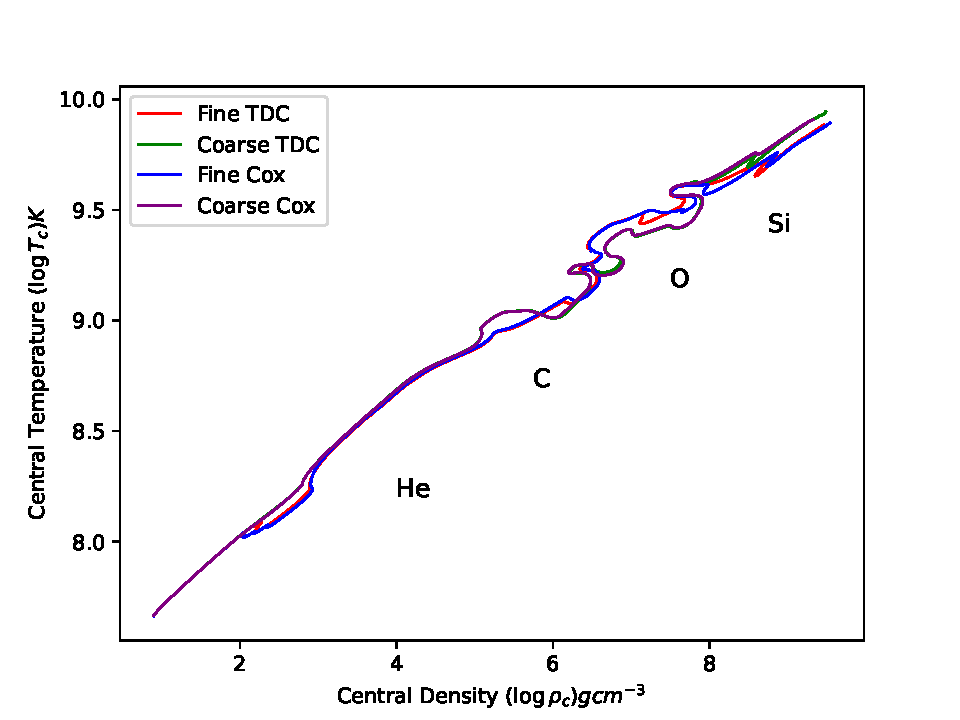
\includegraphics[width=0.9\linewidth]{TcRc_Compare}
    \caption{Graph of central temperature (\gls{Tc}) against central density (\gls{rhoc}), plotted from $35\%$ H in the core for four models varying by timestepping and mixing theory. Locations of burning stages are labelled (label locations based on \citealp{Maeder09}).}
    \label{fig:TcRc_Compare}
\end{center}
\end{figure}

Likewise, Figure \ref{fig:HDR_Compare} shows a similar story, where all models show consistent \gls{lum} by \gls{Teff} relationships 
up to \gls{ZAMS}. Notably, however, the greater resolution led to increased differences between \gls{MLT} and \gls{TDC} after this point.

The similarities seen in the \gls{HRD} before core collapse were likely a result of how the envelope and core were decoupled at this point (see Section \ref{sec:AdvancedEvolution}).
%\begin{figure}[H]
\begin{center}
    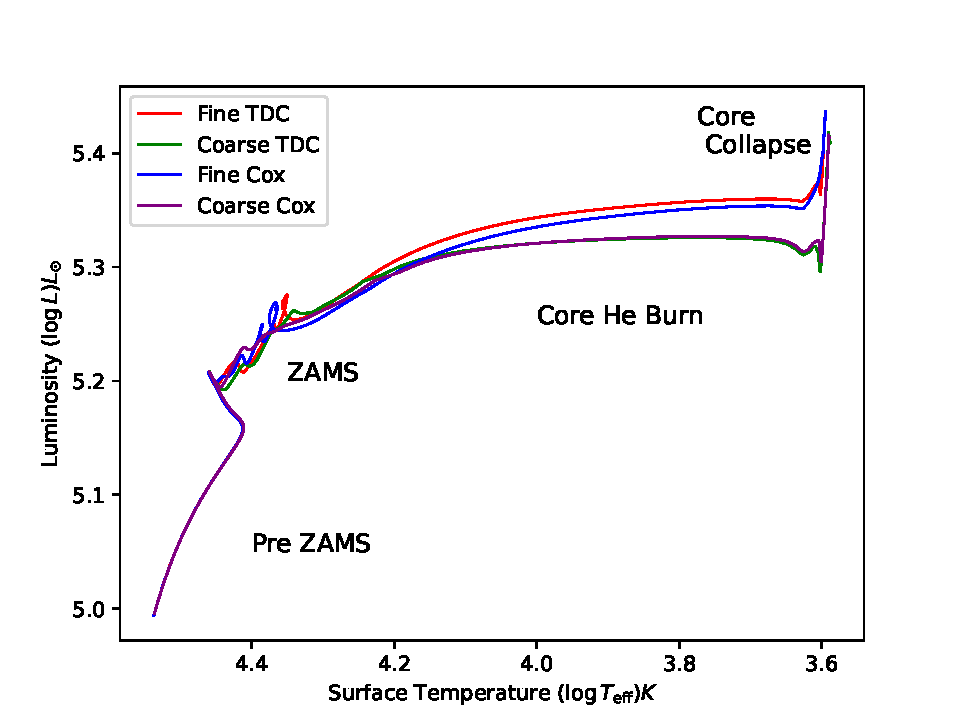
\includegraphics[width=0.9\linewidth]{Figures/HDR_Compare.pdf}
    \caption{\gls{HRD} showing change in luminosity by surface temperature of four models from H-burning at $35\%$ core He, varying only by mixing theory and resolution (Fine = high resolution, Coarse = test run resolution). Important stages are labelled (where ZAMS = zero age main sequence; label location after \citealp{Maeder09}).}
    \label{fig:HDR_Compare}
\end{center}
\end{figure}